\documentclass[12pt]{article}
\usepackage[margin=1in]{geometry}
\usepackage{amssymb}
\usepackage{enumitem}
\usepackage[hidelinks]{hyperref}
\usepackage{tikz}
\usetikzlibrary{arrows.meta,positioning,shapes.geometric}


\setlength{\parindent}{0pt}
\setlength{\parskip}{0.25\baselineskip}
\setlist[itemize]{
  noitemsep,
  nosep,
  topsep=2pt,
  partopsep=0pt,
  parsep=0pt,
  before=\vspace{-\parskip}
  }
\setlist[enumerate]{
noitemsep,
nosep,
  topsep=2pt,
  partopsep=0pt,
  parsep=0pt,
  before=\vspace{-\parskip}
  }

\title{WORKING TITLE:\@ The Unknowing}
\author{}
\date{}

\begin{document}
\maketitle
\tableofcontents

\setcounter{section}{-1}
\section{Postmodern and Metamodern}

\subsection{Metamodern}

\begin{itemize}
  \item sincerity rises from irony (or through)
  \item reconstructs everything while questioning
  \item hopeful but not foolish
  \item meanings are rebuilt, not deconstructed
  \item “maybe something matters” vibe
\end{itemize}

Metamodern oscillates between realism and romanticism.

Metamodern doubts, but it’s not nihilistic.

Emotions are exposed.

Self-aware vulnerability.

Meanings are not rejected and the search of truths is meaningful.

Even lies can create meanings.

Even a detached person can choose to care (Geralt, Tyson).

References in Metamodern:
\begin{itemize}
  \item create emotional resonance
  \item bridge to meanings
  \item reconnect with the past sincerely (no parody or deconstruction)
  \item irony with belief
  \item they are meaningful, not just ironic
\end{itemize}

Key thing in Metamodern: Reconstruction:
\begin{itemize}
  \item nothing matters → something matters
\end{itemize}

\subsection{Postmodern}

\begin{itemize}
  \item irony and detachment
  \item total deconstruction
  \item “everything is constructed”
  \item references tend to remind the above
  \item truth doesn’t exist
  \item cynical
  \item meanings are undermined — nothing matters
  \item if nothing matters, then one can construct intellectual play with (or without) references
\end{itemize}

\subsection{Key Distinction Between Postmodern and Metamodern}

Postmodern says: “This is an illusion”; metamodern says: “Yes — and I choose to believe in it anyway.”

\begin{center}
\begin{tabular}{p{0.44\textwidth} p{0.44\textwidth}}
  \textbf{Postmodern} & \textbf{Metamodern} \\
  \hline
  deconstruct meaning & reconstruct meaning \\
  expose illusions & live with illusions (not in illusion) \\
  maintain irony & balance irony + sincerity \\
  detach from morality & re-engage morally \\
  undermine emotions & rehabilitate emotions \\
  reject grand narratives (all narratives) & build “soft” personal narratives
\end{tabular}
\end{center}

\subsection{Next Phase (After Metamodern)}

\begin{itemize}
  \item what my belief actually costs?
  \item ethical becomes practical: This is the right thing and here is the price.
  \item not just a system vs an individual, but the system composed of self-aware individuals
\end{itemize}

\subsection{Key Points That Make Literary Fiction}

\begin{itemize}
  \item what part of the self is built out of the lie?
  \item character’s perception must change
  \item probably even language around it
  \item truth arrives as contamination
  \item turn everything — every tiny scene — into a conflict — external or internal; or at least make it psychologically charged
  \item plot twists (clues) should disturb relationships, stakes, memory, language
  \item a protagonist understands the regime but cannot understand themselves outside of it
  \item how do we know
  \item what evidence mean
  \item scenes that do not advance the plot but deepen the wound
  \item an attempt to interpret a world that already colonised its methods of interpretation
  \item the “investigation” must produce artistic pressure, not just suspense
  \item every scene must have double weight: move the surface action and deepen the novel’s argument about perception by damaging the protagonist’s self-understanding, changing the reader’s relationship to the language (in broader term, I guess) of the book
  \item a protagonist’s perception has been trained by the society
  \item pressure the protagonist from chapter 1
  \item the protagonist cannot stay psychologically static even in the first part of the book
  \item any referential unit work as an image itself
  \item match tone of the reference
\end{itemize}

\subsection{Modern Dystopia Structure}

\begin{enumerate}[label=\Roman*.]
  \item World introduction + protagonist
  \item The rebellion
  \item The defeat of the rebellion
\end{enumerate}

\textbf{My corrections}:
\begin{enumerate}[label=\Roman*.]
  \item The protagonist is a part of the system
  \item Step by step he realises that the system is fucked up
  \item He could never help to realise that he’s still a part of the system nonetheless
\end{enumerate}

\textbf{The rebellion}: It is not crushed by the authorities; it fails because not that many people actually care about it.

People are passive and ignorant — that’s the biggest problem.

\section{Core Premise}

\textbf{How it looks from the first glance}: Engineered epistemic inequality.

→ Society is intentionally divided into:
\begin{itemize}
  \item those who understand reality — wizards
  \item those who do not
\end{itemize}

Most people were deprived of knowledge, thus:
\begin{itemize}
  \item no longer understand how the world works
  \item refer to technology as “magic”
  \item (?) cannot vote
  \item live on universal basic income
  \item exist primarily as consumers, thus are used to redistribute the wealth between corporations
  \item even most CEOs don't understand how the system is actually structured: there is no evil mastermind or Big Brother: the system balances itself
  \item thus they believe they're actually `making money', not redistributing them
\end{itemize}

Wizards:
\begin{itemize}
  \item retain full education
  \item design and run society
  \item form scientific, economic, political and partially art elites
  \item are employed by corporations
  \item retain political power
\end{itemize}

\textbf{But under the hood}: Civilization chose comfort over understanding. This includes the protagonist leaving the academia.

Key idea:
\begin{itemize}
  \item Knowledge was not taken away
  \item It was voluntarily abandoned (2030s–2040s)
  \item Over generations → complete epistemic collapse (“magic” worldview)
  \item many people, protagonist included, chose finance over science not because of money, but because it’s easier; money is just the driver
\end{itemize}

\section{Themes}
\subsection{Conceptions}
\begin{itemize}
  \item Voluntary surrender of education: prefer simple answers to complex questions
  \item Comfort over understanding
  \item Higher layer: Not magic — illusion. Illusion vs reality:
  \begin{itemize}
    \item illusion of democracy
    \item illusion of choice
    \item illusion of knowledge
  \end{itemize}
  \item People as capital-flow instruments
  \item Conception: forced labour shall be forbidden, which implies that most of us live in concentration camps, in fact
  \item Abundance → austerity
  \item “The poor and the stupid” support power and the rich: “They should know better”
  \item Corporations manipulate belief → control capital flow: The corporations use lies and consiracy theories to shift money flows, ie. To shift people to buy their products. And politicians sort of do the same
  \item Absolute power must be destroyed, not administered
  \item Elderly people stuck to their seats
  \item Educated people can’t bear how the commoners fall into conspiracy theories, yet they themselves often fall into conspiracy theories and superstitions themselves without noticing it:
  \begin{itemize}
    \item mock conspiracy theories
    \item yet fall into their own
  \end{itemize}
  \item Educated people want to educate people/masses; they want everybody to be like them, to live in their paradigm
\end{itemize}

\subsection{Repetitative}
\subsubsection{The Ceiling}

Mention several times that the ceiling in the protagonist’s flat is quite high—higher than in Victorian houses, certainly higher than in Georgian houses. A spider lives in the corner he can’t even reach.

His brother lives in a new-ish house with low ceilings; the antagonist lives in the old house—or a new-build—with very high ceilings, yet he still dreams about spending nights under the skies.

\subsubsection{Authorial Fallibility and Metafiction}

\begin{itemize}
  \item Have several references that are clearly wrong — to show that the author is no better than his subjects.
  \item Try to have some author that dies midbook — to troll the death of the author concept.
\end{itemize}

\section{Plot Structure}

\begin{enumerate}
  \item Illusion of mass rebellion
  \item Actually:
  \begin{itemize}
    \item corporations fighting via justified misinformation
    \item one greedy CEO (or even a lower-level corporate rat) wants to shift the market this way
  \end{itemize}
  \item The real rebellion is rising among the educated class, though fails because the commons don’t care about it. The protagonist gets dragged into this rebellion, he goes to common people with the ideas and stuff. But this rebellion was also staged by the corporates fighting each other, because ‘chaos is a ladder’.
  \item Protagonist:
  \begin{itemize}
    \item joins
    \item tries to educate masses
    \item teaches at old school
    \item some children engage with real science
  \end{itemize}
  \item Revelation: rebellion staged by corporations and the antagonist
  \item Collapse: masses turn against him
\end{enumerate}

How educated people fall for this (or another) conspiracy:
  \begin{itemize}
    \item free speech
    \item liberalism
    \item take back control and give it to the people
    \item give people knowledge — they choose conspiracy
    \item create a new (fake) woke class
  \end{itemize}
  
(?) The corporation wants to launch a new “thinking device,” “knowledge bank,” or smth like that. The educated see their chance in it; the mob use it for conspiracy.

\begin{center}
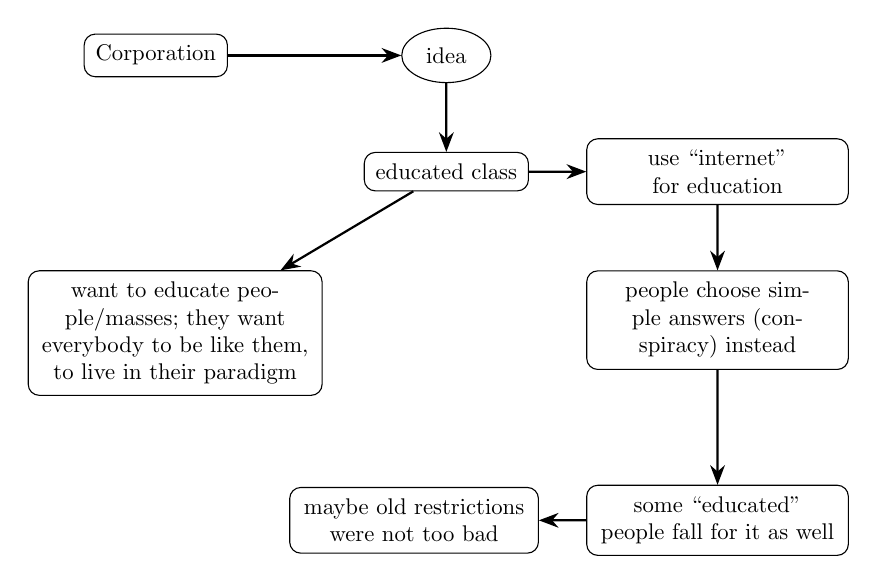
\begin{tikzpicture}[
  scale=0.82,
  transform shape,
  >={Stealth[length=2.5mm]},
  box/.style={draw, rounded corners, align=center, inner sep=5pt},
  idea/.style={draw, ellipse, align=center, inner sep=5pt},
  flow/.style={->, thick}
]
  \node[idea] (idea) at (0,0) {idea};
  \node[box] (corporation) at (-4.5,0) {Corporation};
  \node[box] (educated) at (0,-1.8) {educated class};
  \node[box, text width=4.2cm] (educate) at (-4.2,-4.3)
    {want to educate people/masses; they want everybody to be like them, to live in their paradigm};
  \node[box, text width=3.7cm] (internet) at (4.2,-1.8)
    {use “internet” for education};
  \node[box, text width=3.7cm] (answers) at (4.2,-4.1)
    {people choose simple answers (conspiracy) instead};
  \node[box, text width=3.7cm] (fall) at (4.2,-7.2)
    {some “educated” people fall for it as well};
  \node[box, text width=3.5cm] (restrictions) at (-0.5,-7.2)
    {maybe old restrictions were not too bad};

  \draw[flow] (corporation) -- (idea);
  \draw[flow] (idea) -- (educated);
  \draw[flow] (educated) -- (educate);
  \draw[flow] (educated) -- (internet);
  \draw[flow] (internet) -- (answers);
  \draw[flow] (answers) -- (fall);
  \draw[flow] (fall) -- (restrictions);
\end{tikzpicture}
\end{center}

\begin{center}
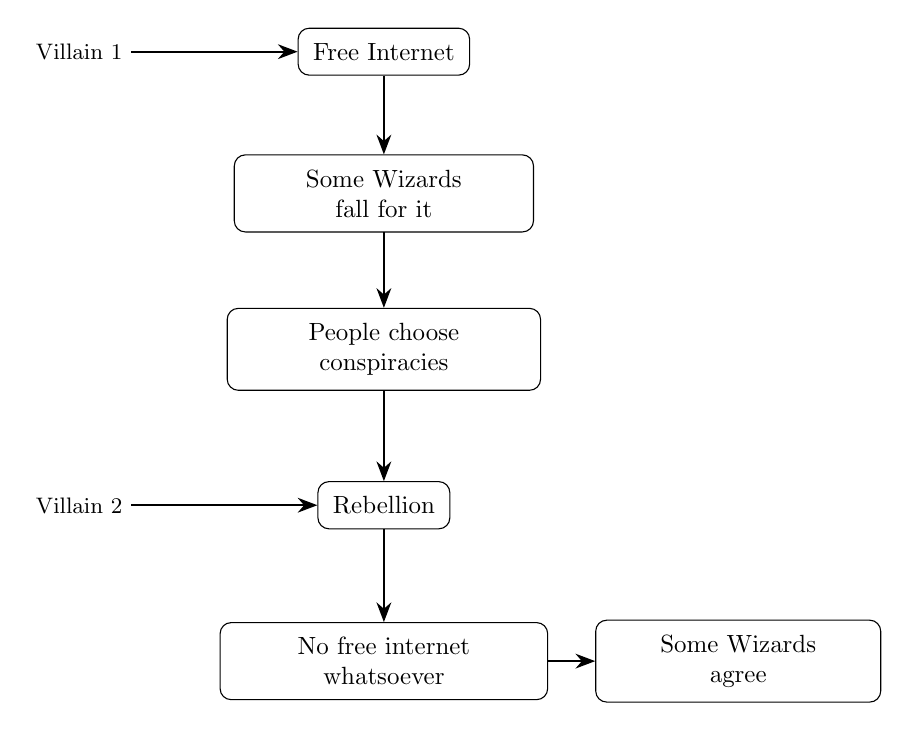
\begin{tikzpicture}[
  scale=0.9,
  transform shape,
  >={Stealth[length=2.5mm]},
  box/.style={draw, rounded corners, align=center, inner sep=6pt},
  flow/.style={->, thick},
  side/.style={font=\small, align=center}
]
  \node[box] (free) at (0,0) {Free Internet};
  \node[box, text width=3.8cm] (wizards) at (0,-2.0)
    {Some Wizards\\fall for it};
  \node[box, text width=4.0cm] (conspiracies) at (0,-4.2)
    {People choose\\conspiracies};
  \node[box] (rebellion) at (0,-6.4)
    {Rebellion};
  \node[box, text width=4.2cm] (nofree) at (0,-8.6)
    {No free internet\\whatsoever};
  \node[box, text width=3.6cm] (agree) at (5.0,-8.6)
    {Some Wizards\\agree};
  \node[side] (villain1) at (-4.3,0)
    {Villain 1};

  \node[side] (villain2) at (-4.3,-6.4)
    {Villain 2};

  \draw[flow] (villain1) -- (free);
  \draw[flow] (free) -- (wizards);
  \draw[flow] (wizards) -- (conspiracies);
  \draw[flow] (conspiracies) -- (rebellion);
  \draw[flow] (villain2) -- (rebellion);
  \draw[flow] (rebellion) -- (nofree);
  \draw[flow] (nofree) -- (agree);

\end{tikzpicture}
\end{center}

The leader of the underground works for one of the corporations. He pulls everything off at some point and the protagonist and a few more educated people are left alone with the mob they were trying to save. The cops don’t even bother to step in.

Potential ending: he is killed by the parents of the children he’s teaching as ‘heretic’. He might have a chance to escape, but he stops to wave his best pupil to look away and that’s how the crowd gets him. So failure, but with a glimpse of hope. Potential location for this scene: Charing Cross.

He gets beaten explicitly in the liver. By a man called `Desert' (as `Deser Eagle' EAGLE!).

\section{History}

\begin{itemize}
  \item The story is set some 100--150 years from now
  \item around present day, maybe in 2030s or 2040s, people were not deprived of knowledge, they gave it up themselves. Not everyone of course, but those who wanted to carry on with science and engineering were accepted in the ruling class (the most unrealistic part, given our governments, but this is something a smart ruler would do and I want my villain to be smart), but the vast majority — and this is the bottom line — gave up the knowledge voluntarily. And it took a few generations to come to ‘magic’.
  \item Progress slowed down a bit, but it’s not critical. Don’t make it obvious until late.
  \item \ldots{}they voted for extra charges (fees) when leaving TV on and not using it.
  \item In the 60-s half of population of several states died of measles because they weren’t vaccinated, because a few decades before there was a mass social panic that vaccines cause ADHD. It wasn’t the vaccines, though; it wasn’t even true ADHD, it were social networks and the algorithms.
  \item Progress slowed but not critically (hidden until late).
\end{itemize}

\section{Social Structure}

\begin{enumerate}
  \item The Masses (“Commoners”)
  \begin{itemize}
    \item No deep education
    \item Basic literacy + arithmetic only
    \item Believe technology is magic: Smartphone works on magic, computers work on magic, rockets fly on magic, etc.
    \item Consume content and products
    \item Often name children after brands.
    \item Allowed:
    \begin{itemize}
      \item small services (repairs, beauty, arts)
      \item entertainment production (books, music, standups, even theatres)
    \end{itemize}
  \end{itemize}

  \item The Educated Elite (“Wizards”)
  \begin{itemize}
    \item Either generational or
    \item Selected via early testing
    \item Educated in special schools → universities
    \item Become scientists, engineers, corporate employees
    \item Often employed by corporations
    \item Those generational (‘old knowledge’) are not forced into science and leadership, though it’s far easier for them to get there
  \end{itemize}

  \item Corporations (True Power)
  \begin{itemize}
    \item Control production, knowledge, and narratives
    \item People running corporations use misinformation and conspiracy theories
    \item Governments:
    \begin{itemize}
      \item funded by corporate taxes
      \item operate in corporate interest
    \end{itemize}
    \item Internet is restricted and censored and stuff
  \end{itemize}

  \item Government
  \begin{itemize}
    \item Minimal role
    \item Income: corporate taxation
    \item Incentive: austerity
  \end{itemize}
\end{enumerate}

\begin{itemize}
  \item Many people still live in old houses augmented with modern technologies and materials installed by robots/androids.
  \item People usually meet up in virtual rooms where their avatars can interact like real humans. All streamed directly to their minds via neurochips.
  \item Physical meetings are elite, e.g. Endowment (uni gatherings)
\end{itemize}

\section{Education System}
\subsection{General Schools}

Schools. Well, these are quite different. They are not mandatory, yet most people still want to ship their children somewhere for the solar day. They teach basic stuff: the language and the arithmetics, but that’s pretty much it. The rest they teach are brands and technologies — which products you can consume. But also empathy — crime is expensive, so it's better to teach people how not to become criminals, how to respect each other, respect the private space including sexual space — also because unplanned pregnancies cannot be genetically controlled and this would be more expensive for the healthcare system. And the only source of income governments are left with are corporate taxes — literally corporates chipping in — so they are interested in the austerity as is.

There are no human teachers -- only robots, but there are some volunteering overseers.

\begin{itemize}
  \item Not mandatory
  \item Function as childcare and consumer training centers
  \item Teach:
  \begin{itemize}
    \item language
    \item arithmetic
    \item brands \& products
    \item empathy (to reduce crime)
    \item sexual boundaries (to avoid costly pregnancies)
  \end{itemize}
\end{itemize}

\subsection{The 6-Year-Old Test (MANDATORY)}

Purpose:

Identify talented children for elite education

Name candidates:
\begin{itemize}
  \item Fulcrum
  \item Vocation
  \item Klesis
  \item Ahvana
  \item Dharma
\end{itemize}

\subsection{Elite Schools}

\begin{itemize}
  \item Full education restored
  \item Pipeline to universities and thus corporate roles
\end{itemize}

\section{Underground}

\subsection{Underground Universities}

\begin{itemize}
  \item Teach real science and society
  \item Example The Underground University of London is situated in the underground. One of the campuses — Charing Cross station.
\end{itemize}

\subsection{Underground Movement}

\begin{itemize}
  \item Educated resistance
  \item No enforcement power
  \item Opposes:
  \begin{itemize}
    \item corporations (authorities)
    \item ignorant masses (scum)
  \end{itemize}
  \item Maybe in the underground the protagonist is asked to chose a nickname. He choses ‘Dustfinger’.
\end{itemize}

\subsection{Marginal Resistance (The Resistance of the Poor)}

The resistance of the poor: some people form the marginal resistance — they don’t understand a fuck how the system works, but they feel deprived and they want to take power. This movement is not enspired by the authorities. Probably the only resistanse movement that is not enspired by the authorities.

\begin{itemize}
  \item Do not understand system
  \item Feel deprived
  \item Want power
  \item Not controlled by authorities (initially)
  \item Eventually:
  \begin{itemize}
    \item manipulated against educated class
    \item absorb defectors from underground
  \end{itemize}
\end{itemize}

They claim they want 'The Truth', but it's a lie (most of them sincirely lie themselves, though). They want everyone else to accept 'their truth'.

A conspiracy theory about some Luddite group that wants to destroy serving/working robots, for people to do working services for other people — to bring back human interaction (puke). No such thing exists.

But those in power trick them to oppose the underground universities and the middle class (the wizards who were not born, but passed the \textless{}\textgreater{} like the protagonist) instead. With time going, many people from the underground university turn to this movement because it offers simple answers right now, not in the future after significant mental effords. People defect fast and it’s these people who beat up the protagonist in the very end.

Low-IQ conspiracy theory about thought control via brain-chips. Leading to the conclusion that for thought control you don’t need some devices; you don’t even need resourceful propaganda — ignorance is enough.

There is also another conspiracy: the protagonist’s elite bosses financed the “free internet conspiracy,” so they build a “common folk riot” for the government to ban any free internet that might come up. The protagonist fights this conspiracy/riot thing and wins.

\section{Technology}

\subsection{Some Technologies, Producs and Corporations}

\begin{itemize}
  \item Sheep Inc → AI system
  \item Aerocab → transport
  \item Neural interfaces:
  \begin{itemize}
    \item Most Wizards interact with AI via ‘thought-tokens’ (‘mind-tokens’) — not words, not images, but concepts; most non-wizards interact via words like we do.
  \end{itemize}
  \item Immersive reality (games + porn)
  \item Ads transmitted into dreams. For those who have no premium subscription, of course.
  \item People use “The Guidance Service” — literally the state-controlled AI — need a better, maybe more magical term for it; global internet is the ancient ruin.
  \item Genetic augmentation of children: someone convinced it’s cheaper than treat them the entire life
  \item Robots/androids:
  \begin{itemize}
    \item perform all manual labor
    \item not fully anthropomorphic
    \item can do most if not all manual labor: gas checks, electricity installation, plumbering, repairs, etc.
    \item no unions, fatigue, illness, pregnancy
  \end{itemize}
\end{itemize}

Repeated phrasing variants:
\begin{itemize}
  \item Robots don’t get tired, don’t get sick, don’t get pregnant, and they don’t join unions.
  \item Robots don’t tire, don’t fall ill, don’t get pregnant — and they never join a union.
  \item Robots never tire, never fall ill, never bear children — and never form unions.
\end{itemize}

\subsection{Space Infrastructure}

\begin{itemize}
  \item Moon:
  \begin{itemize}
    \item datacentres
    \item superconducting supercomputers
    \item quantum computers (possibly)
    \item solar panels
    \item maybe: dig materials for solar panels on the Moon, thus manufacture the panels on the Moon too
  \end{itemize}
  \item Data packet loss exists but manageable
\end{itemize}

\subsection{In-Progress Tech (more easter eggs really)}

\begin{itemize}
  \item Fusion reactor
  \item Graphene transistor
\end{itemize}

\section{Various}

\subsection{Battersea Power Station}

I definitely need a scene at the Battersea Power Station; 1984 was filmed there, maybe the Wall as well. Somebody says it was the first mall in the UK. Someone gives a presentation in the cinema with their face magnified on the screen?

\subsection{Old and New Towers of London}

\begin{itemize}
  \item Old Tower of London:
  \begin{itemize}
    \item means there is New Tower of London
    \item good chapter name
    \item New Tower of London is an office building — shall be read as “prison”
  \end{itemize}
\end{itemize}

\subsection{Estuary Reservation}

There’s an Estuary reservation: a village to protect the Estuary accent after Cockney died out completely. There are several primary schools there, and only kids from families with the right accent are allowed. People are encouraged to stay in the village, but not forced to.

\subsection{Dialogue Fragments}

“You’re in your… what, late twenties? So find yourself a common girl for a night or two.”

“All the common girls of my age are expecting their seconds, or even thirds.”

\section{Characters}

\subsection{Harley Smith}
\subsubsection{General}

\begin{itemize}
  \item Former academic (PhD in Differential Topology)
  \item Quit academia → chose comfort
  \item Now analyst in logistics/food company
  \item Works with chocolate production logistics\\ (cheaper in cold regions like Russia, Canada, Norway and the heat does not affect the taste)
  \item Traits:
  \begin{itemize}
    \item prefers glasses over vision correction (aesthetic choice: looks sexier)
    \item the protagonist tries to help the others, as seeing those less successful makes him less miserable
    \item many people, protagonist included, chose finance over science not because of money, but because it’s easier; money is just the driver
  \end{itemize}
  \item Some phrases:
  \begin{itemize}
    \item “I’m not that kind of wizard, I’m a theorist.”
    \item “How do you do, fellow morlocks.”
  \end{itemize}
\end{itemize}

\begin{itemize}
  \item[\(\checkmark\)] The missing pieces Harley notices:
  \begin{itemize}
    \item how Harley gets introduced to the intellectual resistance
    \item how Harley is connected to the villain
    \item how Harley meets the mob resistance
    \item how Harley is a part of the system (i.e. the knowledge he gave up without noticing)
  \end{itemize}
\end{itemize}

\subsubsection{Harley’s Connection to the Antagonist}

He has to be connected to the protagonist. The easiest way — the protagonist works for his corporation, but this seems lame. What about the endowment evening? — they also share the uni.

\subsubsection{Family and Old Friends}

Brother: Davi (Davidson)
\begin{itemize}
  \item has a child (\textasciitilde{}4 years old)
\end{itemize}

Also show how hard it is for Harley to be with his family and old friends who are all not on the same page with him — and it’s not just the literacy or falling for conspiracies — it’s how they live their lives.

\subsection{The Antagonist}

\subsubsection{Profile}

\begin{itemize}
  \item In his mid–late 50s.
  \item He’s self-made, just like the protagonist.
  \item The villain must be of similar heritage to the protagonist. He’s not entitled, he’s selected; he fought himself through all the steps of the corporate ladder, and yet still he wasn’t appointed CEO — some entitled twat was. So he comes up with his villain plan.
  \item He’s the son/grandson of immigrants.
\end{itemize}

\subsubsection{Motivation}

He realised at some point that he reached his ceiling: no matter how much effort he puts, he won’t be accepted into “elites” — he wasn’t born elite, he was chosen to serve — at the highest level, but serve nonetheless.

He also realises that the “promises of capitalism,” “the capitalistic dream,” is nothing but a lie.

\begin{itemize}
  \item He could have started his own venture, hire a team — it’s not forbidden, but he wouldn’t even acquire big clients, as the markets are saturated by oligopolies.
  \item He tried to follow the rules, reached the ceiling; now his ambition pushes him to cross the rules…
\end{itemize}

\subsubsection{The Antagonist’s Scheme and Key Scenes}

Through the antagonist or otherwise address elderly people stuck to their seats.

When he presents his plan to the Board, some entitled twat (maybe even the CEO himself) says, “Shall we just raise the prices?” And the profits would be higher than from his masterful plan because of the scale.

Obviously, at some point he must offer the protagonist to join him.

Okay, so his endgame: he wants to bring back free internet, and he secretly builds up infrastructure for it (missing pieces). Then he wants to build the demand, starting with self-educated enthusiasts. The existing educated class is too frail for this purpose, plus there is almost no connection with the common folk: they're too fond of their Ivory Towers. He stimulates underground schools and unis to create connections between educated and uneducated classes. He believes that the free internet would start with educated enthusiasts hungry for information and like-minded people, but once exposed to commercials, brain-rot content would consume it. But he doesn’t care: he wants to sell it to everyone, so brainrot it is.

The corporation would profit silently from the increasing demand of the legacy infrastructure.

One [of] the “dystopian revealing dialogues”: the villain tells the protagonist:

“Knowledge is power,” so they say… Bullshit!… Power is power.

\subsubsection{Family and Elite Access}

Once, a very important business owner invited the antagonist to a dinner and introduced him to his family, including his daughter of similar age. Many years ago, he realised that it was an attempt to bring him into the family—probably the only way to get into the real “elites,” inherit the business, and pass it to his children.

\begin{itemize}
  \item Yes, he needs the family.
\end{itemize}

\subsubsection{Endgame Motivation}

I have two options for his endgame: “human” and “megalomania.”

Human: he wants appreciation, and he wants to be finally taken into the “elites” — this makes him fucking pathetic.

The second one I find more interesting, though much harder to portrait realistically: he wants to disturb the markets and create a new niche he can dominate, and finally step in as an “elite” himself. Petyr Baelish figure.

This can go even deeper: even in this setup he’s still pathetic. He doesn’t want to fight the system; he wants to dominate inside the system — yet another slave who doesn’t want freedom, but slaves of his own.

\subsection{Background Characters}

\subsubsection*{Stavro}

Stavro — he was but a kid when his parents — both software engineers — fled their autocratic Eastern European country in early XXI century — to the UK first, but them moved to the land of the free — to the US for better opportunities and lower taxes. The Antagonist?

\subsubsection*{Lugh}

Surname of someone good, maybe protagonist’s mentor. He’s Irish. Lugh tried to do some good for the common people, but got disappointed and now he’s drinking some vodka with an eagle on it’s logo. Or famous grouse.

\subsubsection*{Matarishvan}

also one of the teachers/mentors who wants to bring (restore) the knowledge back to humanity.

\section{Draft Chapter Structure}

\subsection{Chapter 1 — Wizard}

\begin{itemize}
  \item “You’re a wizard, Harley!”
  \item A 6yo boy receives an invitation from the top school to be trained as a wizard.
  \item Oi, young boy, learn the rules like your bruver before you.
\end{itemize}

\subsection{Chapter 2 — Missing Pieces}

\begin{itemize}
  \item Lives in Brixton Rise — block houses built some 50 years ago.
  \item Works as analyst
  \item Notices missing inventory
  \item Nobody gives a fuck
  \item As a data-science professional, I want to invent a way to describe EDA in a cool, modern and sexy way—even if for a single scene.
\end{itemize}

\subsection{Chapter 3 — Endowment}

Meeting with old coursemates at the Uni — UCL that became the University of London. Can you believe there was once more than a 100 unis in the UK. Well, I can believe Edinburgh might have wanted one, but places like Manchester? Why study Russian if you have the translation from all the languages in your earpiece? Meeting occurs in the Orwell house.

\subsection{Chapter 4}

Chapter 4 — meeting with brother? Or back to his missing pieces again?

\section{References and Easter Eggs}

\subsection{Book Censorship Pattern}

Allowed:
\begin{itemize}
  \item 1984
  \item Brave New World
  \item Fahrenheit 451
  \item Player Piano
\end{itemize}

Banned:
\begin{itemize}
  \item Tolkien
  \item Remarque — A Sparkle of Life
\end{itemize}

The books are banned if they have hope. And they’re not really banned banned, it’s just harder to get them.

\subsection{Easter Eggs}

\begin{itemize}
  \item Player Piano in museum
  \item Wizard → sorcerer (an American student calls him so) → Warlock (deal with evil power) →  he accepts he’s a warlock and the warlock goes to war
  \item \ldots{}much better genius than Henry Ford or Elon Musk (turns out to be a witted nazi)
  \item F-word → fascism
  \item Khaluy like about the commons, but truly for the educated enablers of the system
  \item oligarch (actually greek — mention Aristotelis)
  \item “Sputnik” never used
  \item Life is not a textbook with the correct answers at the end. Not even to odd-numbered problems.\ (give the answers in the second half of the book)
  \item Some stupid person suggest the theory that if Homer was English, he would have named his character Journathan
  \item Zuck avatar thing: the billionaire uses an AI avatar for something he doesn’t treat as important or to train conversations with him before actual conversations
  \item St James — is the one who fucked his sister?
  \item In to deep — deep state
  \item Farage → Forage → Furage → Fourage -- PM who got rid of the teachers because they were too expensive
  \item Chapter name: Middle Ground. Win or lose -- you don't die (at least)
  \item several “[Promethei?]” → “[Ouroborosis?]”
  \item Ouroborosis — at least he has a proper fuck; except he fucks himself...
\end{itemize}

\subsection{Music References}

For the novel from Metallica:

\begin{itemize}
  \item The Unforgiven (all 3 verses)
  \item Iron Mainden ‘Brave New World’ — twisted wings — swans in St James’ park.
  \item Pink Floyd’s first name: Sigma 6. And \(\sigma\) is the standard deviation; 6 sigmas — fucking lot from the mean.
  \item Scum of Brixton.
  \item David Bowie is from Brixton → Man Who Sold the World → face to face with David Bowie (the mirror).
  \item The return of Ziggy Stardust?
  \item Whoever who chose easy over right (business/finance over science) is a man who sold the world.
  \item Can also mention Nirvana somewhere around here.
  \item Master of Puppets — not heroin, not the drugs, but money, corporate world.
  \item He drops his breakfast (sausage) on a mirror board (why? but a cool reference maybe not for Chapter 2). In the office?
\end{itemize}

\section{IDENTIFIED GAPS}

\subsection{Worldbuilding Gaps}

\begin{itemize}
  \item Final name 
  \item Mechanics of 6-year-old test
  \item Exact structure of government vs corporations
  \item Naming of robots/androids
\end{itemize}

\subsection{Plot Gaps}

\begin{itemize}
  \item Mechanism of protagonist discovering truth
  \item Timeline of rebellion stages
  \item Role of corporate agent leader (identity, arc)
  \item How underground operates day-to-day
\end{itemize}

\end{document}
